\begin{figure}[H]
\centering

\includegraphics[width=\textwidth]{fcde904bdc7a185ad1a9ea71b12161c7.jpg}
% \caption{}
\label{}
\end{figure}

\begin{exercise}
\begin{figure}[H]
\centering

\includegraphics[width=\textwidth]{hw12-2025052821.png}
% \caption{}
\label{}
\end{figure}
\end{exercise}
See Apostol.
\begin{figure}[H]
\centering
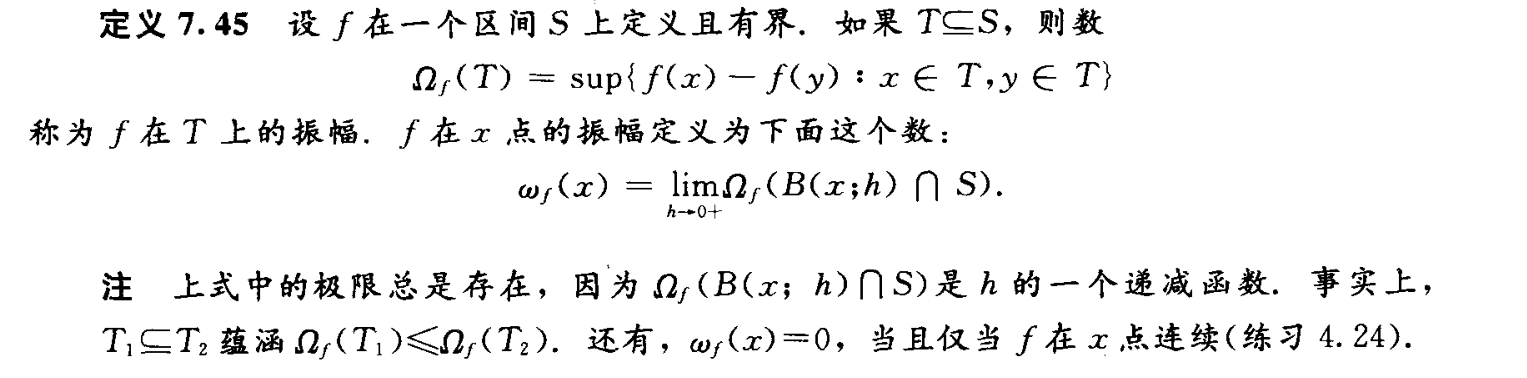
\includegraphics[width=\textwidth]{hw12-2025052822.png}
% \caption{}
\label{}
\end{figure}

\begin{figure}[H]
\centering

\includegraphics[width=\textwidth]{5-hw12-2025052821.png}
% \caption{}
\label{}
\end{figure}
\begin{figure}[H]
\centering
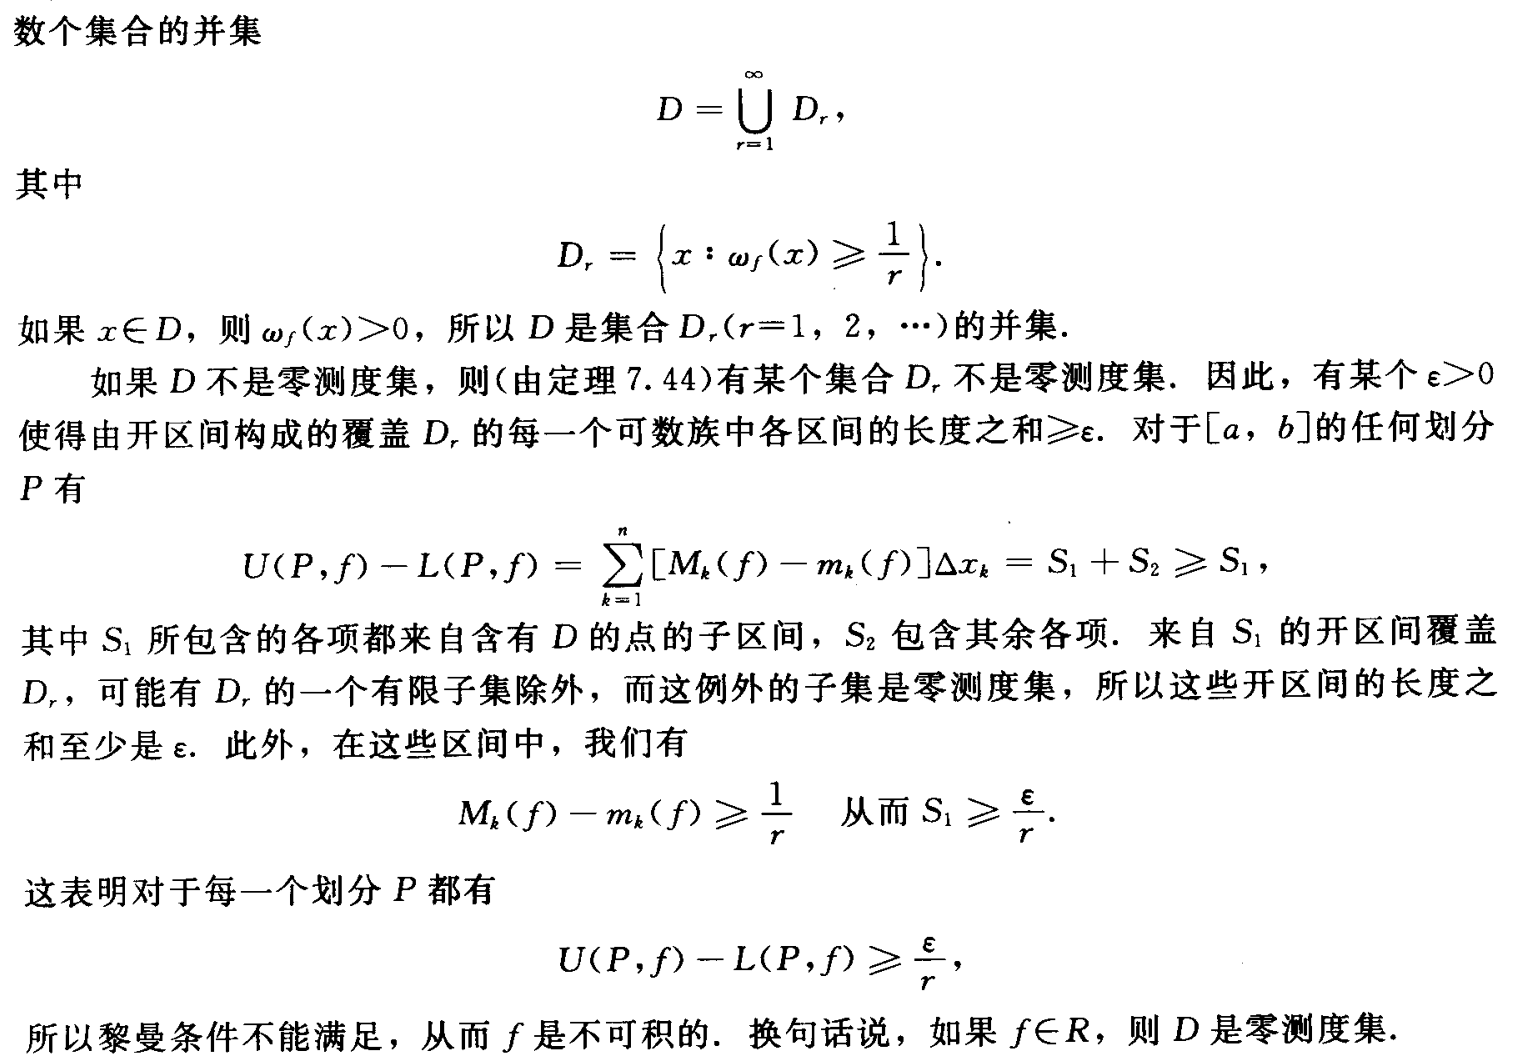
\includegraphics[width=\textwidth]{6-hw12-2025052821.png}
% \caption{}
\label{}
\end{figure}
\begin{figure}[H]
\centering
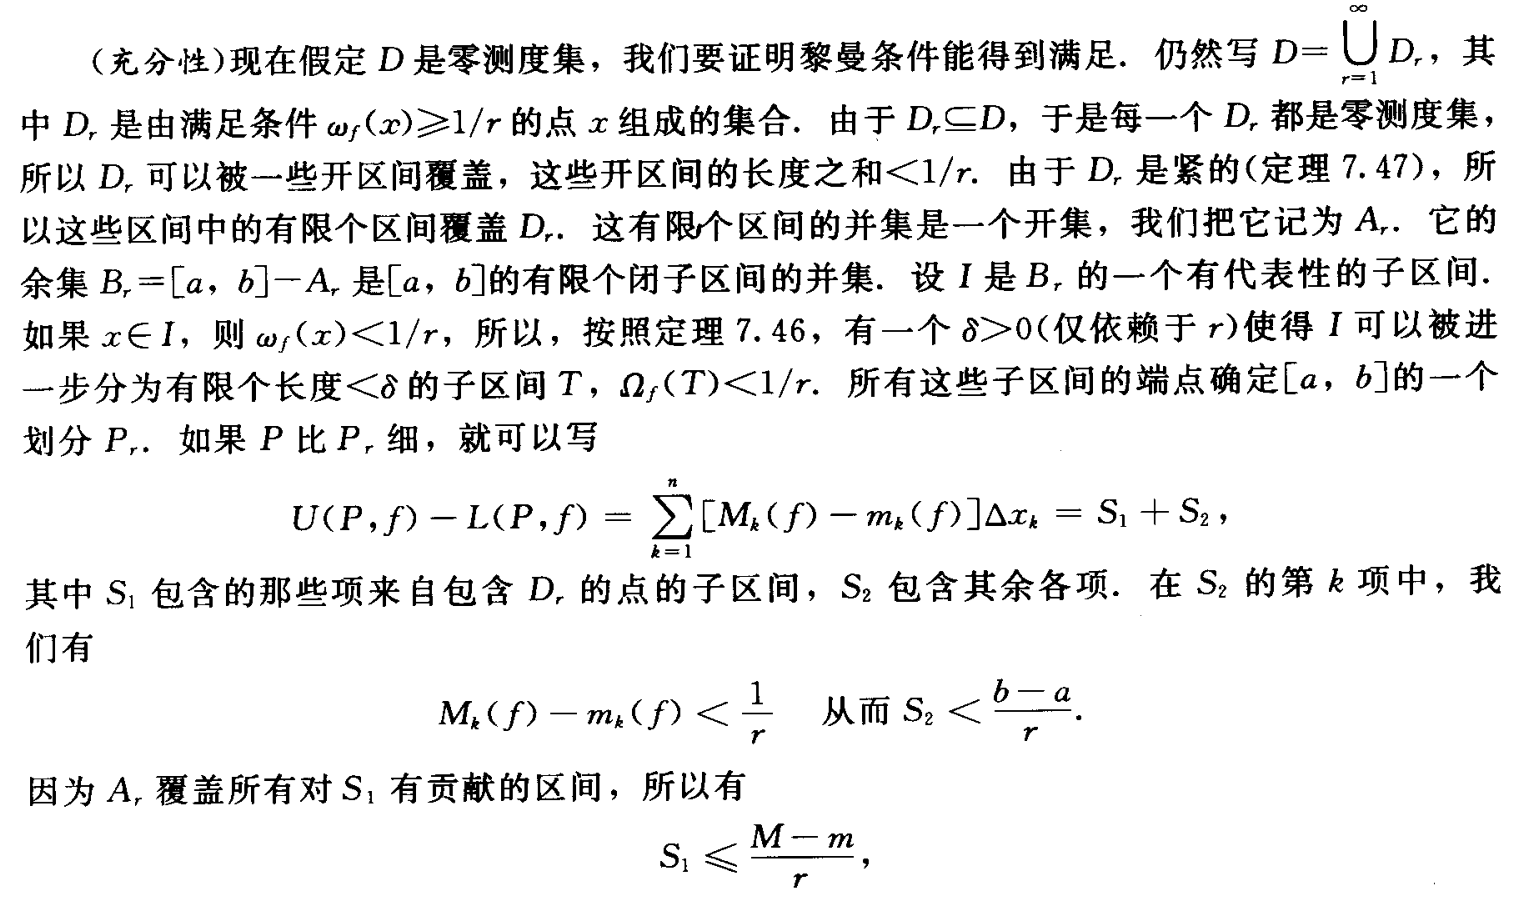
\includegraphics[width=\textwidth]{7-hw12-2025052821.png}
% \caption{}
\label{}
\end{figure}
\begin{figure}[H]
\centering

\includegraphics[width=\textwidth]{8-hw12-2025052821.png}
% \caption{}
\label{}
\end{figure}

\begin{exercise}
\begin{figure}[H]
\centering

\includegraphics[width=\textwidth]{1-hw12-2025052821.png}
% \caption{}
\label{}
\end{figure}
\end{exercise}
不妨设 $0<m\leq g\leq M$, 于是 $g$ 和 $\frac{1}{g}$ 有相同的不连续点,由于 $f,g$ 在 $[a,b]$ 黎曼可积,故 $f, g$ 有界且不连续点集为零测集. 于是 $\frac{f}{g}$ 的不连续点为零测集,且 $\lvert f/g \rvert\leq\frac{1}{m}\lvert f \rvert$ 故 $f/g$ 有界,故 $f/g$ 黎曼可积.

\begin{exercise}
\begin{figure}[H]
\centering

\includegraphics[width=\textwidth]{2-hw12-2025052821.png}
% \caption{}
\label{}
\end{figure}
\end{exercise}
\begin{figure}[H]
\centering
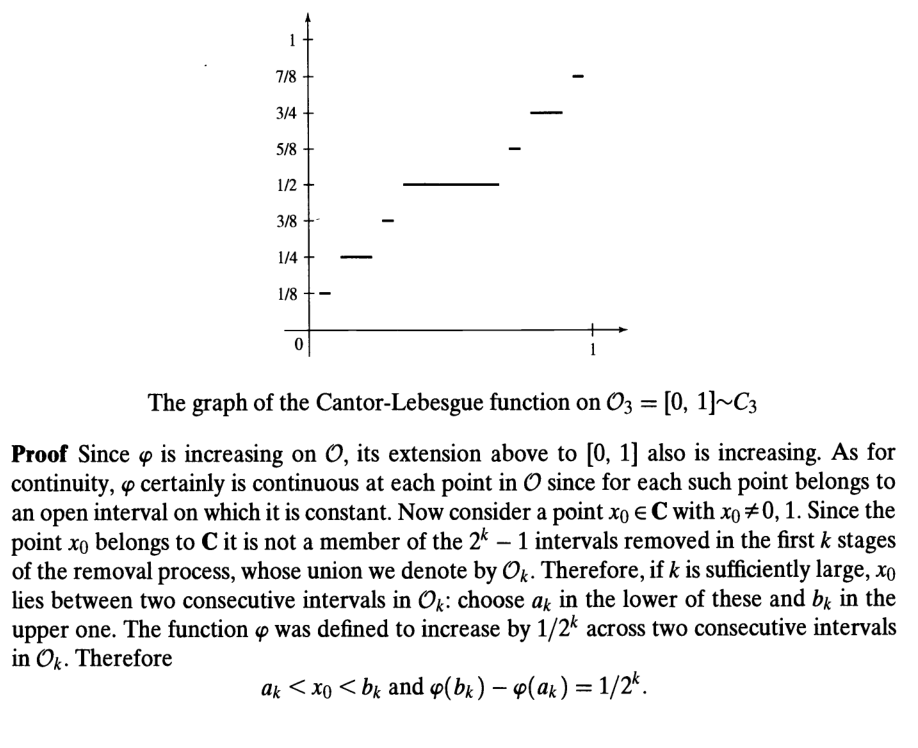
\includegraphics[width=\textwidth]{1-hw12-2025052822.png}
% \caption{}
\label{}
\end{figure}
\begin{figure}[H]
\centering
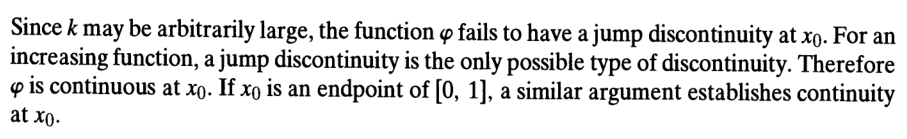
\includegraphics[width=\textwidth]{2-hw12-2025052822.png}
% \caption{}
\label{}
\end{figure}

\begin{exercise}
\begin{figure}[H]
\centering

\includegraphics[width=\textwidth]{3-hw12-2025052821.png}
% \caption{}
\label{}
\end{figure}
\end{exercise}
\begin{figure}[H]
\centering
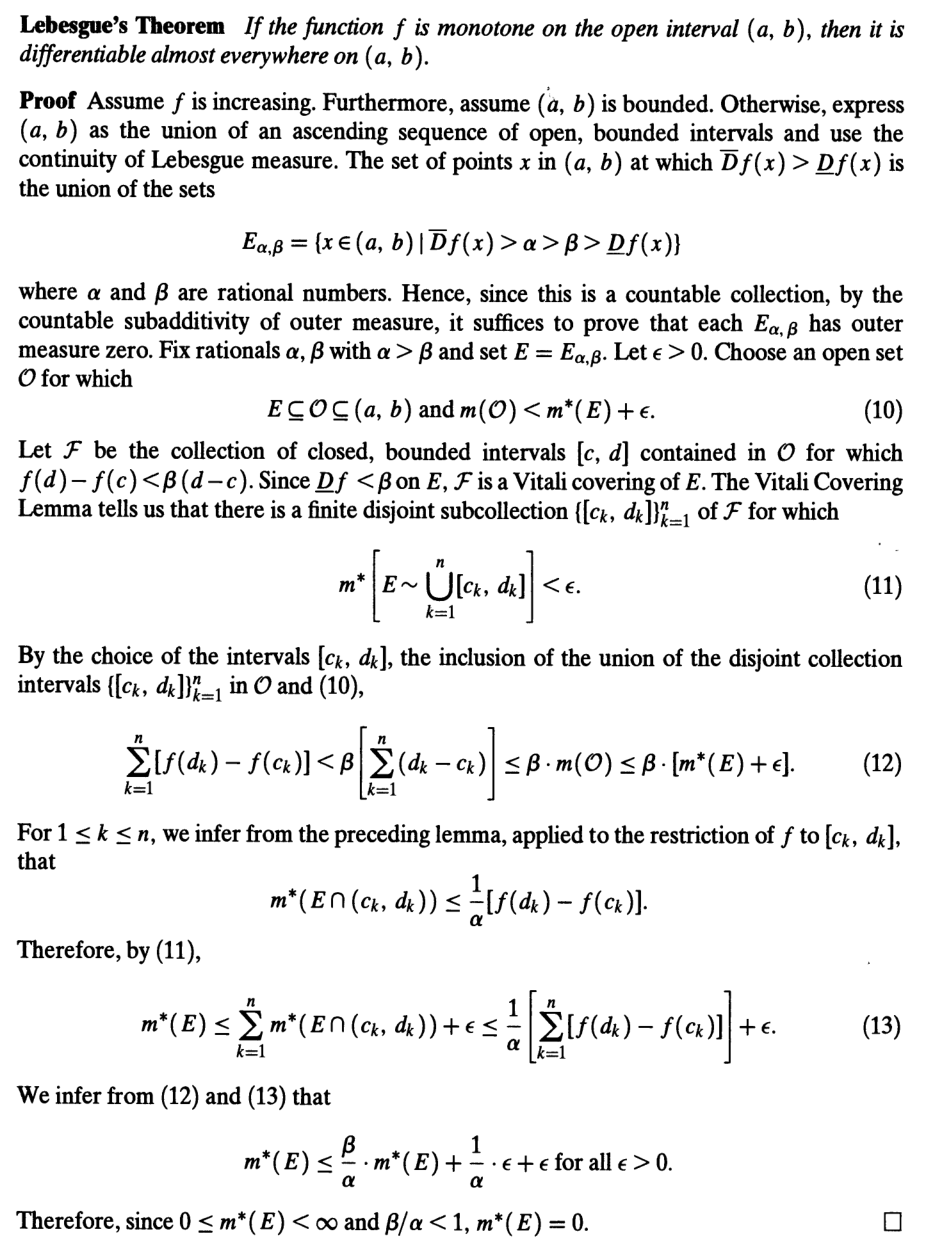
\includegraphics[width=\textwidth]{3-hw12-2025052822.png}
% \caption{}
\label{}
\end{figure}

\begin{exercise}
\begin{figure}[H]
\centering

\includegraphics[width=\textwidth]{4-hw12-2025052821.png}
% \caption{}
\label{}
\end{figure}
\end{exercise}
\begin{figure}[H]
\centering
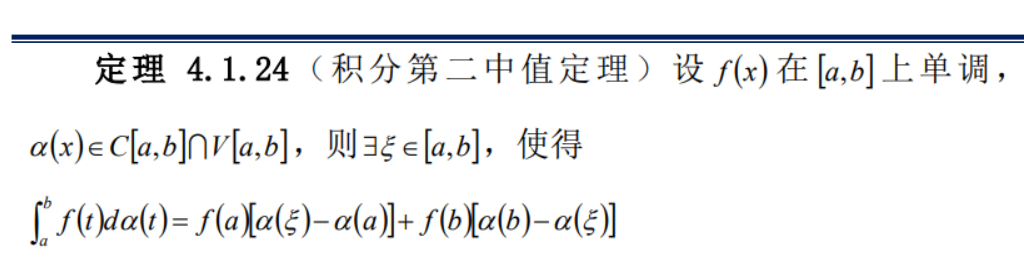
\includegraphics[width=\textwidth]{4-hw12-2025052822.png}
% \caption{}
\label{}
\end{figure}

考虑连续函数
\[
g(x)=f(a)[\alpha(x)-\alpha(a)]+f(b)[\alpha(b)-\alpha(x)]-\int_{a}^{b} f(t) \, \mathrm{d}\alpha(t)
\]
则
\[
g(a)=f(b)[\alpha(b)-\alpha(a)]-\int_{a}^{b} f(t) \, \mathrm{d}\alpha(t)=\int_{a}^{b} \underbrace{ [f(b)-f(t)] }_{ \geq 0 } \, \mathrm{d}\alpha(t) \geq 0 
\]
\[
g(b)=f(a)[\alpha(b)-\alpha(a)]-\int_{a}^{b} f(t) \, \mathrm{d}\alpha(t) =\int_{a}^{b} \underbrace{ [f(a)-f(t)]  }_{ \leq 0 }\, \mathrm{d}\alpha(t)\leq 0 
\]
由介值定理可知:存在 $\xi\in[a,b]$ 使得
\[
g(\xi)=0
\]
即
\[
\int_{a}^{b} f(t) \, \mathrm{d}\alpha(t)=f(a)[\alpha(\xi)-\alpha(a)]+f(b)[\alpha(b)-\alpha(\xi)]
\]